\PID 
Одредити развој сигнала
$v(t) = V_0 |\sin(\upomega_0 t)|$ у Фуријеов ред на његовом основном периоду, применом 
својстава и табличних трансформација. $V_0$ је позната константа. 

\RESENJE 
На свом периоду $T = \dfrac{2\uppi}{\upomega_0}$ дати сигнал се може представити производом синусоиде 
$x(t) = V_0 \sin(\upomega_0 t)$ 
и симетричне биполарне поворке правоугаоних импулса $r(t)$ као 
$v(t) = x(t) \cdot r(t)$, где је 
$r(|t| < T) = \begin{cases}
    -1, t < 0 \\
    1, t > 0
\end{cases}.$ 
Применом својства о множењу у временском домену \refs{s:ctfs:conv}, спектар траженог сигнала се 
онда одређује конволуцијом $V[k] = X[k] \ast R[k]$. 

Таблично одређивање спектра поворке $r(t)$ урађено је као II начин решења задатка \ref{z:pravougani_po_def},
а релевантан резултат је 
\begin{equation}
    R[k] = -\jj \dfrac{2}{k\uppi} \begin{cases}
        1, & k\text{ непарно} \\
        0, & k\text{ парно}
    \end{cases}.
\end{equation}
Спектар синосоиде се може одредити, на пример формалним развојем до експоненцијалних чланова па је 
\begin{equation}
    x(t) = V_0\sin(\upomega_0 t) = 
    V_0 \dfrac{\ee^{\jj\upomega_0 t} - \ee^{-\jj\upomega_0 t}}{\jj2} = 
    \underbrace{-\jj\dfrac{V_0}{2}}_{X[1]} \ee^{\jj(1)\upomega_0 t} + \underbrace{\jj\dfrac{V_0}{2}}_{X[-1]} \ee^{\jj(-1)\upomega_0 t} ,
\end{equation}
односно $X[k] = \jj\dfrac{V_0}{2}\left(\updelta[k+1] - \updelta[k-1]\right)$. Конволуција се израчунава 
применом одговарајућих својстава\footnote{Користи се особина 
$x[n] \ast \updelta[n - n_0]  = x[n-n_0]$, $n_0 = \const$.} као 
\begin{eqnarray}
    \hspace*{-20mm}
    V[k] &=& X[k] \ast R[k] = 
    \jj\dfrac{V_0}{2}\left(\updelta[k+1] - \updelta[k-1]\right) \ast -\jj \dfrac{2}{k\uppi} 
    \begin{cases}
        1, & k\text{ непарно} \\
        0, & k\text{ парно}
    \end{cases}  \\[5mm]
    &=&
    \dfrac{V_0}{\uppi} \left(
        \dfrac{1}{k} 
        \left\{
        \begin{array}{ll}
            1, & k\text{ непарно} \\
            0, & k\text{ парно}
        \end{array}
        \right\}
        \ast \updelta[k+1]
        +
        \dfrac{1}{k} 
        \left\{
        \begin{array}{ll}
            1, & k\text{ непарно} \\
            0, & k\text{ парно}
        \end{array}
        \right\}
        \ast \updelta[k-1] 
    \right) \\
    &=&
    \dfrac{V_0}{\uppi}
    \left(
        \dfrac{1}{k+1}
        \left\{
        \begin{array}{ll}
            1, & k+1\text{ непарно} \\
            0, & k+1\text{ парно}
        \end{array}
        \right\}
        -
        \dfrac{1}{k-1}
        \left\{
        \begin{array}{ll}
            1, & k-1\text{ непарно} \\
            0, & k-1\text{ парно}
        \end{array}        
        \right\}
    \right) 
\end{eqnarray}
Пошто операција $\pm 1$ мења парност целог броја, добијени израз се може поједноставити чиме се добија да 
коначни резултат има само парне спектралне компоненте и то
\begin{equation}
    V[k] = \dfrac{V_0}{\uppi} \left(
        \dfrac{1}{k+1}
        -
        \dfrac{1}{k-1}
    \right) \begin{cases}
        1, & k\text{ парно}, \\
        0, & k\text{ непарно}
    \end{cases}
    = 
    -\dfrac{2V_0}{\uppi} \dfrac{1}{k^2 - 1}\begin{cases}
        1, & k\text{ парно}, \\
        0, & k\text{ непарно}
    \end{cases}
\end{equation}
График добијеног спектра приказан је на слици \ref{fig:\ID.abssinVk}.

\begin{figure}
    \centering 
    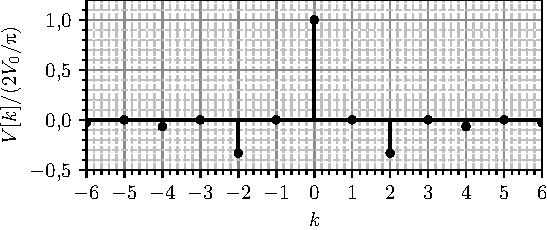
\includegraphics{fig/abs_sin_Vk.pdf}
    \caption{Уз резултат задатка.}
    \label{fig:\ID.abssinVk}
\end{figure}
Приказани резултат представља Фуријеов развој датог сигнала 
на периоду $T_{\rm F} = \dfrac{2\uppi}{\upomega_0}$. 
У овом спектру се може приметити да је сваки други (сваки непаран) члан раван нули. 
То је индикативно\footnote{Иако јесте индикативно, то није правило. На пример, као у задатку 
\ref{z:pravougani_po_def} добија се сигнал са само непарним хармоницима, развијен на основном периоду.} 
томе да је добијен развој на \textit{умношку} основног периода, као 
из својства \refs{s:ctfs:mT0}. 
То је последица да сигнал $|\sin(\upomega_0 t)|$ има двоструко мањи период од сигнала 
$\sin(\upomega_0 t)$. На основу поменутог својства, развој на основном периоду се добија уклањањем 
уметнутих нула, односно, заменом $k \mapsto 2k$, чиме се добија спектар без нула 
\begin{equation}
    V'[k]_{(T_{\rm F} = T_0)}
    = 
    -\dfrac{2V_0}{\uppi} \dfrac{1}{4k^2 - 1}
\end{equation}